% This file was created with tikzplotlib v0.10.1.
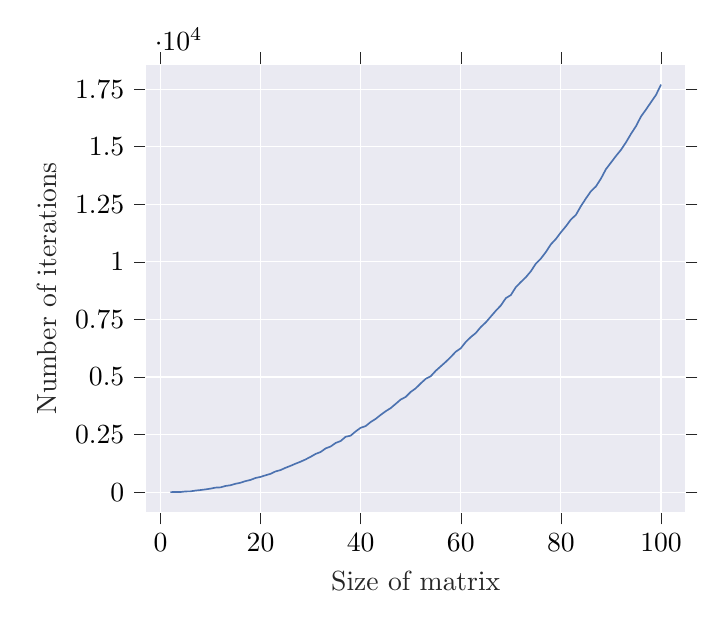
\begin{tikzpicture}

\definecolor{darkslategray38}{RGB}{38,38,38}
\definecolor{lavender234234242}{RGB}{234,234,242}
\definecolor{steelblue76114176}{RGB}{76,114,176}

\begin{axis}[
axis background/.style={fill=lavender234234242},
axis line style={white},
mark options={mark size=2.5pt, line width=1.5pt},
minor xtick={},
minor ytick={},
tick align=outside,
title style={align=center},
x grid style={white},
xlabel=\textcolor{darkslategray38}{Size of matrix},
xmajorgrids,
xmajorticks=false,
xmajorticks=true,
xmin=-2.9, xmax=104.9,
xtick style={color=darkslategray38},
xtick={-20,0,20,40,60,80,100,120},
y grid style={white},
ylabel=\textcolor{darkslategray38}{Number of iterations},
ymajorgrids,
ymajorticks=false,
ymajorticks=true,
ymin=-884, ymax=18586,
ytick style={color=darkslategray38},
ytick={-2500,0,2500,5000,7500,10000,12500,15000,17500,20000}
]
\addplot [semithick, steelblue76114176]
table {%
2 1
3 9
4 6
5 31
6 35
7 69
8 92
9 120
10 153
11 198
12 208
13 269
14 301
15 365
16 409
17 480
18 532
19 616
20 663
21 733
22 796
23 901
24 960
25 1059
26 1144
27 1238
28 1324
29 1422
30 1535
31 1660
32 1745
33 1900
34 1983
35 2136
36 2221
37 2405
38 2455
39 2637
40 2797
41 2870
42 3046
43 3183
44 3356
45 3514
46 3651
47 3835
48 4023
49 4136
50 4354
51 4509
52 4725
53 4922
54 5036
55 5271
57 5659
58 5870
59 6099
60 6249
61 6525
62 6734
63 6912
64 7171
65 7374
67 7879
68 8107
69 8425
70 8560
71 8903
72 9125
73 9334
74 9593
75 9926
76 10144
77 10430
78 10764
79 10996
80 11285
81 11546
82 11841
83 12042
84 12423
85 12756
86 13069
87 13278
88 13618
89 14027
91 14599
92 14866
93 15192
94 15560
95 15894
96 16315
97 16616
98 16938
99 17252
100 17701
};
\end{axis}

\end{tikzpicture}
